%% Slide 7.
\begin{frame}
\frametitle{Il modello di P.Morillo et al.}
\begin{itemize}[<+->]
\item
$3$ server, di cui uno contrassegnato come principale;
\item
$180$ client che controllano un avatar nel mondo virtuale;
\item
una rete che connette i client ai server (che sono tra loro interconnessi);
\item
un ambiente virtuale (Virtual Environment);
\item
un metodo ed un file di partizionamento che il server principale utilizza per
suddividere il carico tra i server.
\end{itemize}
\end{frame}

%% Slide 8.
\begin{frame}
\frametitle{Il modello di P.Morillo et al.}
\begin{center}
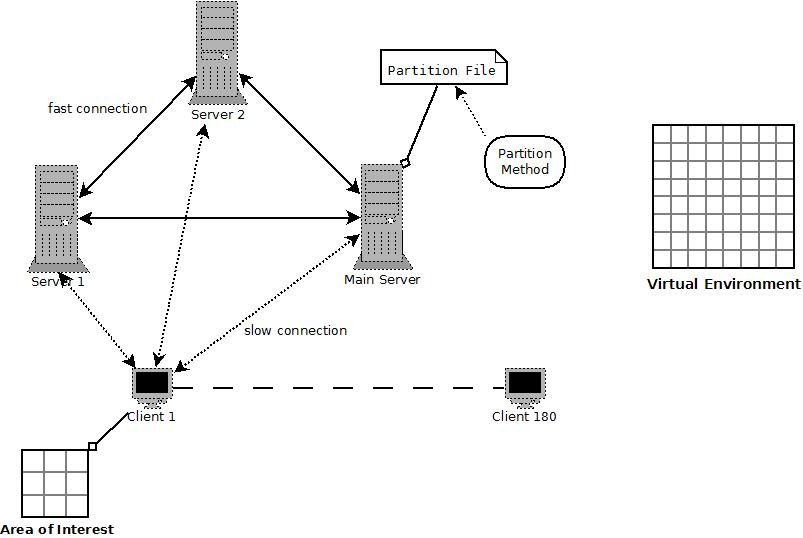
\includegraphics[scale=.45]{schema.jpeg}
\end{center}
\end{frame}


%% Slide 9.
\begin{frame}
\frametitle{Il modello di progetto}
\begin{itemize}[<+->]
\item
$1$ Main Server che si occupa del login dei client e della gestione
dell'ambiente simulato;
\item
$k \in \{1, \ldots, 9\}$ Server di Partizione che si occupano di gestire i
messaggi tra client ed aggiornare il Main Server;
\item
$n$ client che controllano un distinto avatar nel mondo virtuale;
\item
una rete WAN simulata che connette i client ai server;
\item
una rete LAN simulata che connette i server con una struttura ad anello
unidirezionale;
\item
un ambiente virtuale (\texttt{VirtualEnvironment});
\item
un metodo di partizionamento statico, dipendente dal numero di Server di
Partizione, che il Main Server utilizza per suddividere il carico.
\end{itemize}
\end{frame}

%% Slide 10.
\begin{frame}
\frametitle{Il modello di progetto}
\begin{center}
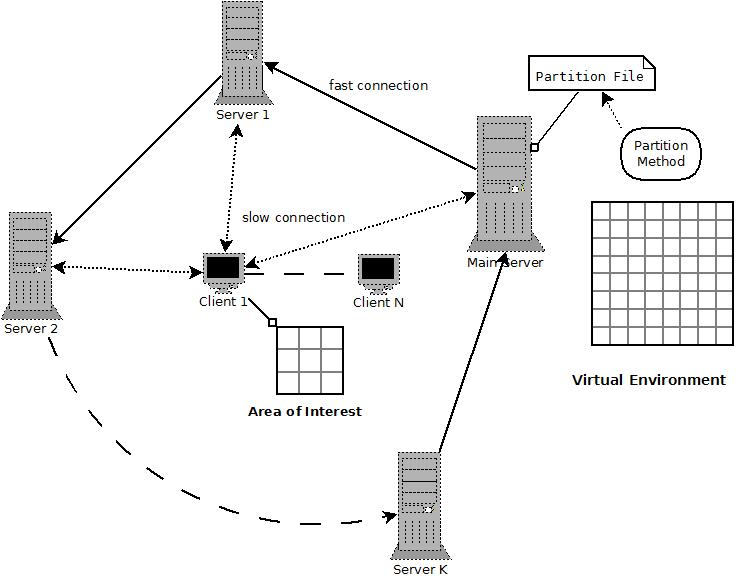
\includegraphics[scale=.45]{schemaRing.jpeg}
\end{center}
\end{frame}
